\chapter{Other Work}
\label{chap:other}

Below is a brief synopsis of other work undertaken over the past two years.

\section{Layer Based Analysis of the Kidneys}

The vast majority of analysis of renal \ac{MRI} data is based around defining \ac{ROI} within the kidneys. While this method has provided excellent results, it is by no means perfect as these \ac{ROI} need to be manually defined, leading to human bias, or defined by an automated method which, as outlined in Chapter \ref{chap:ML}, can be difficult to generalise.\\

Taking inspiration from the analysis pipelines used by neuroimagers \cite{self_benchmarking_2019, muckli_contextual_2015, waehnert_anatomically_2014}, a method of dividing the kidneys into layers of equal thickness was developed. This method uses a three-dimensional FreeSurfer mesh on the surface of the kidney \cite{dale_cortical_1999} and levelsets to produce a map of how far each voxel is from the surface. From this map it is possible to place voxels into layers of any thickness. An example of this method being applied to both the brain and an ex-vivo kidney sample can be seen, figures \ref{fig:layers_brain} and \ref{fig:layers_kidney} respectively.\\

One of the main challenges in transferring this technique is coping with the reduced \ac{FOV} that comes with body imaging. Given that the method essentially asks how far is each voxel from the closes vertex on the mesh, if the mesh has a large hole in it where the slices stop covering the kidney, then the quantitative nature of this depth map is compromised.\\

\begin{figure}[H]
	\centering
	\begin{subfigure}[c]{0.47\textwidth}
		\centering
		\includegraphics[height=1\textwidth]{Other/Layers/mri_to_roi_to_surf_Artboard_5.eps}
		\caption{}
		\label{fig:layers_brain}
	\end{subfigure}
	\hfill
	\begin{subfigure}[c]{0.47\textwidth}
		\centering
		\includegraphics[height=1\textwidth]{Other/Layers/kidney_levelsets-02.eps}
		\caption{}
		\label{fig:layers_kidney}
	\end{subfigure}
	\caption{(\subref{fig:layers_brain}) A depth mask of the brain. Lighter areas are deeper inside the brain. (\subref{fig:layers_kidney}) A depth mask applied to a quantitative $T_1$ map.}
	\label{fig:layers_example}
\end{figure}

This levelset method was compared to two other methods of producing layers in the kidneys, a two-dimensional and a three-dimensional version of the \ac{TLCO} method \cite{piskunowicz_new_2015, milani_reduction_2017}. Each method was tested with a volume that included the entire kidney, and a cropped volume that only included the central section of the kidney, simulating the reduced \ac{FOV} that is common in body imaging. The layers generated were the applied to a $T_1$ map with the mean and standard deviation of $T_1$ in each layer being plot, Figure \ref{fig:layers_comp}.

\begin{figure}[H]
	\centering
	\begin{subfigure}[c]{0.47\textwidth}
		\centering
		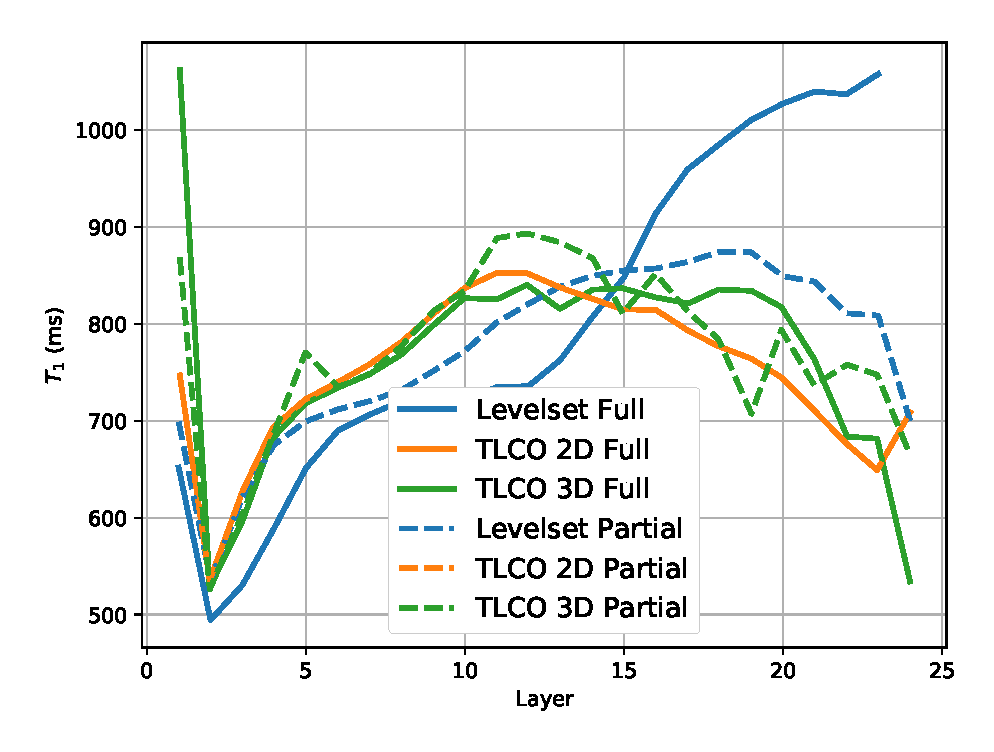
\includegraphics[width=1\textwidth]{Other/Layers/T1_crop.eps}
		\caption{}
		\label{fig:layers_t1_comp}
	\end{subfigure}
	\hfill
	\begin{subfigure}[c]{0.47\textwidth}
		\centering
		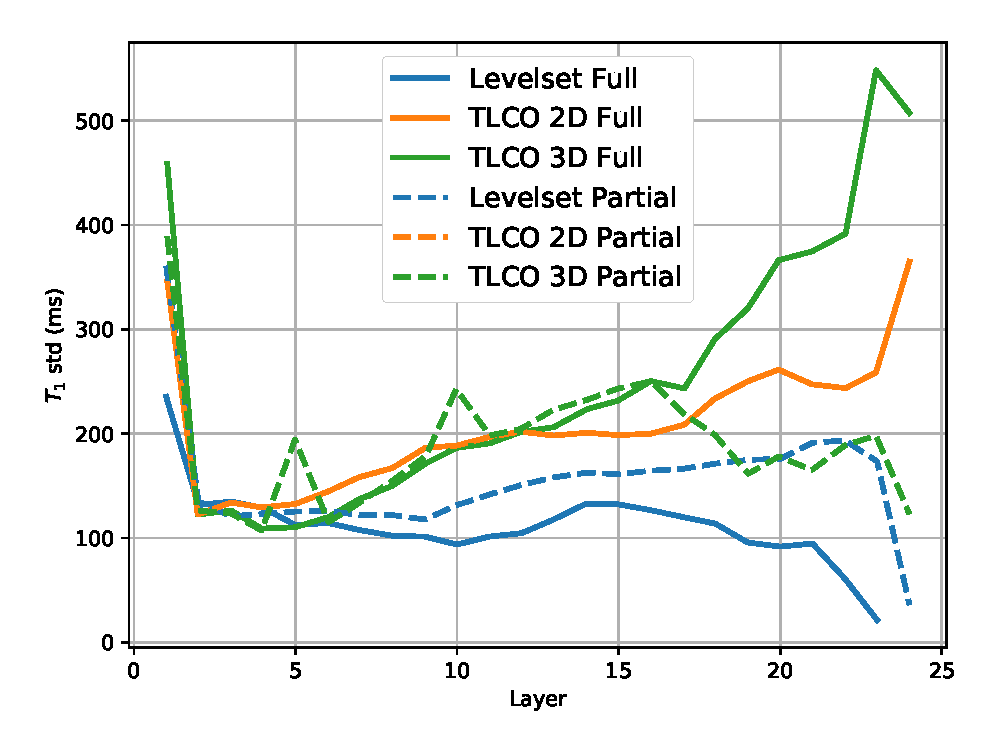
\includegraphics[width=1\textwidth]{Other/Layers/T1_std_crop.eps}
		\caption{}
		\label{fig:layers_t1_std_comp}
	\end{subfigure}
	\caption{(\subref{fig:layers_t1_comp}) The mean $T_1$ within each layers produced by each of the three methods when processing either the full volume of the kidney or only the central slices. (\subref{fig:layers_t1_std_comp}) The standard deviation of the $T_1$ within the layers produced by each method.}
	\label{fig:layers_comp}
\end{figure}

In Figure \ref{fig:layers_t1_std_comp} we can see that the layers output by the levelset method when applied to a full volume dataset produce the minimum standard deviation, this means the layers are the most anatomically sensible as a smooth transition of $T_1$ is expected with depth in the kidney and therefore the variance in each layer should be relatively small. Given this method produces the most realistic layers, other methods will be compared to it.\\

Neither of the \ac{TLCO} methods manage to capture the increase in $T_1$ that can be seen deeper in the kidney. They also have a much larger standard deviation per layer for deeper layers than the levelset method implying that the layers produced are a mixture of cortex and medulla. When comparing the performance of each method with only a partial volume of kidney, the levelset method produces the results that are closes to that of the full volume levelset.\\

Given this method can be used both in-vivo and on ex-vivo samples, they will make for an interesting additional analysis pipeline for the work in Chapter \ref{chap:Neph}.

\newpage
\section{Diffusion Tensor Imaging in the Kidneys}
\label{sec:dti}
As part of the nephrectomy protocol, Chapter \ref{chap:Neph}, we want to be able to assess the microstructure of the kidneys, one avenue to pursue for this is the use of \ac{DTI}. \ac{FA} has been shown to correlate with \ac{GFR} \cite{liu_chronic_2015} and mean tract length is an indicator of ureteropelvic junction obstruction \cite{delgado_pilot_2019} showing that tractography can be used to assess renal structure.\\

One of the major hurdles to overcome in developing a renal \ac{DTI} protocol for this study was correction of both \ac{EPI} readout distortions and eddy current induced distortions. This was achieved using a pipeline based around \ac{FSL}'s topup \cite{andersson_how_2003, smith_advances_2004} and eddy \cite{andersson_integrated_2016} routines. Key acquisition parameters for the sequence are 64 directions arranged over a whole spherical shell to assist with eddy current correction, this whole acquisition is then repeated with the opposite phase-encode direction to enable \ac{EPI} distortion correction. A b-value of 600 s/mm$^2$ is used. \ac{FA} maps are generated using \ac{FSL} and tractography is processed using an in-house pipeline developed using the Dipy Python library \cite{garyfallidis_dipy_2014}.\\

Using this pipeline, images such as those in figures \ref{fig:dti_tracts} and \ref{fig:dti_fa} could be produced. This protocol is now ready to be used on patients undergoing a nephrectomy.

\begin{figure}[H]
	\centering
	\includegraphics[width=.9\textwidth]{Other/DTI/img5c.png}
	\caption{Example tractography generated using the above protocol.}
	\label{fig:dti_tracts}
\end{figure}

\begin{figure}[H]
	\centering
	\includegraphics[width=.55\textwidth]{Other/DTI/dti_FA.png}
	\caption{An example \ac{FA} map generated using the protocol above.}
	\label{fig:dti_fa}
\end{figure}

%\subsection{Apparent Diffusion Coefficient Mapping}
\newpage
\section{Designing Novel MR Phantoms using Additive Manufacturing}

Phantoms used in the field of \ac{MRI} are generally limited to blocks of doped agar \cite{hattori_development_2013} or arrays of liquids of known properties as used in Section \ref{subsec:neph_t2_mapping}. While these types of phantom are useful, they have remained largely unchanged for many years. With the advent of modern manufacturing techniques such as \ac{AM} far more complex phantoms could be designed and built relatively inexpensively.\\

We plan to begin by validating the manufacturing process using a phantom similar to one designed by Berry et al \cite{berry_3d_2017}, Figure \ref{fig:am_hex_phantom}. These phantoms restrict the direction in which the fluid within them can diffuse leading to a higher \ac{FA} for the phantoms with smaller tubules. A technical drawing of one of these proposed phantoms can be seen in appendix \ref{app:fa_phantom}. These small structures would be very difficult and costly to produce before recent developments in \ac{AM}.

\begin{figure}[H]
	\centering
	\includegraphics[width=.7\textwidth]{Images/Other/AM/50um_Hexagonal_2.png}
	\caption{A render of one of the proposed phantoms, in this case each small hexagon is 50 $\mu$m in diameter with a 10 $\mu$m wall separating them.}
	\label{fig:am_hex_phantom}
\end{figure}

Extending this concept, we intend to print a phantom to simulate fibre crossing, appendix \ref{app:fiber_crossing_phantom}. This phantom contains small tubules, half of which always remain in the same direction, the other half of which gradually rotate though forty five degrees. This phantom therefore simulates multiple angles of fibres crossing found in-vivo and should enable the verification of multiple \ac{DTI} tractography reconstruction algorithms, something that has only been performed using somewhat crude phantoms until now \cite{perrin_validation_2005}.\\

A final proposal is to use custom printed phantoms to investigate the accuracy of flow measurements in the kidneys. Similar work has been carried out in other areas of the body \cite{canstein_3d_2008, anderson_validation_2014} however, no such investigation has been done on renal vessels. We propose to begin with a basic flow phantom, Figure \ref{fig:am_flow_render} and appendix \ref{app:flow_phantom}, and verify that the \ac{MRI} measurements correlate well with those predicted using \ac{CFD}, Figure \ref{fig:am_flow_cfd}, before moving onto more complicated geometry of the renal blood vessels comparing in-vivo, ex-vivo and in-silico results.

\begin{figure}[H]
	\centering
	\begin{subfigure}[c]{0.47\textwidth}
		\centering
		\includegraphics[height=0.95\textwidth]{Other/AM/Four_Branch.png}
		\caption{}
		\label{fig:am_flow_render}
	\end{subfigure}
	\hfill
	\begin{subfigure}[c]{0.47\textwidth}
		\centering
		\includegraphics[height=0.95\textwidth]{Other/AM/CFD.png}
		\caption{}
		\label{fig:am_flow_cfd}
	\end{subfigure}
	\caption{(\subref{fig:am_flow_render}) The proposed basic flow phantom with branching structure. (\subref{fig:am_flow_cfd}) \ac{CFD} simulations of the flow through the proposed phantom.}
	\label{fig:am_flow}
\end{figure}
